% !TeX program = xelatex
\documentclass[a4paper,10pt]{article}

% ============================================================================
% សន្លឹកកិច្ចការសិស្ស ស-ខ្មៅ (Student Fill-In Worksheet — No-LCD Classroom)
% មេរៀនទី១៧ (១៧.១.១)៖ សញ្ញាណសូលីត និងផ្ទៃក្រឡានៃព្រីស (ត្រូវគ្នា ១០០% នឹង LS_Plan_PRISM_SA.tex)
% ============================================================================
\usepackage[a4paper, left=0.95cm, right=0.95cm, top=0.75cm, bottom=0.90cm, footskip=0.48cm]{geometry}
\usepackage{amsmath}
\usepackage{unicode-math}
\usepackage{fontspec}
\usepackage{array, colortbl}
\usepackage[table]{xcolor}
\usepackage{enumitem}
\usepackage{pifont}
\usepackage{fancyhdr}
\usepackage{lastpage}
\usepackage{tikz}
\usepackage[most]{tcolorbox}
\usetikzlibrary{calc, arrows.meta, angles, quotes, patterns, decorations.markings, babel}

\makeatletter
\let\@expl@@@mark@update@singlecol@structures@@\relax
\makeatother

% ============================================================================
% ការកំណត់ពុម្ពអក្សរ (Cross-Platform Font Resolver)
% ============================================================================
\providecommand{\NGSFindFonts}{%
  \IfFileExists{C:/Windows/Fonts/cambria.ttc}{%
    \def\NGSSysPath{C:/Windows/Fonts/}%
    \def\NGSUserPath{C:/Users/KIT/AppData/Local/Microsoft/Windows/Fonts/}%
  }{%
    \IfFileExists{./fonts/KhmerOSsiemreap.ttf}{\def\NGSSysPath{./fonts/}\def\NGSUserPath{./fonts/}}{%
    \IfFileExists{../fonts/KhmerOSsiemreap.ttf}{\def\NGSSysPath{../fonts/}\def\NGSUserPath{../fonts/}}{%
    \IfFileExists{../../fonts/KhmerOSsiemreap.ttf}{\def\NGSSysPath{../../fonts/}\def\NGSUserPath{../../fonts/}}{%
    \IfFileExists{../../../fonts/KhmerOSsiemreap.ttf}{\def\NGSSysPath{../../../fonts/}\def\NGSUserPath{../../../fonts/}}{%
    \IfFileExists{../../../../fonts/KhmerOSsiemreap.ttf}{\def\NGSSysPath{../../../../fonts/}\def\NGSUserPath{../../../../fonts/}}{%
    \IfFileExists{../../../../../fonts/KhmerOSsiemreap.ttf}{\def\NGSSysPath{../../../../../fonts/}\def\NGSUserPath{../../../../../fonts/}}{%
    \IfFileExists{../../../../../../fonts/KhmerOSsiemreap.ttf}{\def\NGSSysPath{../../../../../../fonts/}\def\NGSUserPath{../../../../../../fonts/}}{%
      \def\NGSSysPath{../../../../../../../fonts/}\def\NGSUserPath{../../../../../../../fonts/}%
    }}}}}}}%
  }%
}
\NGSFindFonts

\setmathfont[Path={\NGSSysPath}, FontIndex=1, Scale=1.02]{cambria.ttc}
\defaultfontfeatures{Ligatures=TeX}

\setmainfont[
  Path={\NGSUserPath},
  Extension=.ttf,
  Script=Khmer,
  BoldFont={KhmerOSsiemreap},
  BoldFeatures={FakeBold=1.8},
  ItalicFont={KhmerOSsiemreap},
  ItalicFeatures={FakeSlant=0.25},
  BoldItalicFont={KhmerOSsiemreap},
  BoldItalicFeatures={FakeBold=1.8, FakeSlant=0.25}
]{KhmerOSsiemreap}

\newfontfamily\muol[Path={\NGSUserPath}, Extension=.ttf, Script=Khmer]{KhmerOSmuollight}
\newfontfamily\TimesEn[Path={\NGSSysPath}, Extension=.ttf, BoldFont={timesbd}, ItalicFont={timesi}, BoldItalicFont={timesbi}]{times}

\XeTeXlinebreaklocale "km"
\XeTeXlinebreakskip = 0pt plus 1pt minus 0.1pt

\definecolor{panelgray}{gray}{0.93}
\definecolor{headgray}{gray}{0.85}

\pagestyle{fancy}
\fancyhf{}
\renewcommand{\headrulewidth}{0pt}
\fancyfoot[L]{\fontsize{8pt}{10pt}\selectfont អនុវិទ្យាល័យព្រះក្រសាំង \en{---} គណិតវិទ្យា ថ្នាក់ទី៨ \en{|} មេរៀនទី១៧ (១៧.១ សញ្ញាណសូលីត និងផ្ទៃក្រឡានៃព្រីស)}
\fancyfoot[R]{\fontsize{8.2pt}{10pt}\selectfont ទំព័រ \en{\thepage\ / \pageref{LastPage}}}

\setlength{\parindent}{0pt}
\setlength{\parskip}{0pt}
\setlength{\tabcolsep}{4pt}

\newcommand{\en}[1]{{\TimesEn #1}}
\newcommand{\enbf}[1]{{\TimesEn\textbf{#1}}}
\newcommand{\unit}[1]{\,\text{\en{#1}}}
\newcommand{\cnum}[1]{\mbox{\fontsize{10pt}{12pt}\selectfont\ding{\numexpr181+#1\relax}}}
\newcommand{\chkbox}{\tikz[baseline=-0.15ex]\draw[black, line width=0.85pt] (0,0) rectangle (0.25cm,0.25cm);}
\newcommand{\blank}[1]{\makebox[#1]{\dotfill}}
\newcommand{\tri}[1]{\ensuremath{\triangle #1}}

\newcommand{\rightbox}[4][0.18]{%
  \draw[black, line width=0.8pt]
    ($(#3)!#1!(#2)$) -- ($($(#3)!#1!(#2)$)+($(#3)!#1!(#4)$)-(#3)$) -- ($(#3)!#1!(#4)$);
}

\newcommand{\secbar}[2]{%
  \vspace{3pt}%
  \begin{tcolorbox}[
    enhanced, sharp corners, colback=headgray, colframe=black,
    boxrule=0.9pt, boxsep=1pt, top=2.5pt, bottom=2.5pt, left=6pt, right=6pt,
    after skip=3pt
  ]
    {\muol\fontsize{9.2pt}{13.5pt}\selectfont #1}\hfill{\fontsize{8.3pt}{11.5pt}\selectfont\textbf{#2}}
  \end{tcolorbox}%
}

\newcolumntype{L}[1]{>{\raggedright\arraybackslash}p{#1}}
\newcolumntype{C}[1]{>{\centering\arraybackslash}p{#1}}

\begin{document}
\fontsize{9.4pt}{13.8pt}\selectfont

% ============================================================================
% ទំព័រទី ១៖ ក្បាលសន្លឹកកិច្ចការ + E1 + E2 (ស្គាល់បាតព្រីស & លាតប្លង់ 2D) + E3 (និយមន័យ & រូបមន្ត)
% ============================================================================
\begin{tcolorbox}[
  enhanced, sharp corners, colback=white, colframe=black,
  boxrule=1.1pt, boxsep=2pt, top=4.5pt, bottom=4.5pt, left=6pt, right=6pt, after skip=5pt
]
  \begin{center}
    {\muol\fontsize{10pt}{14.5pt}\selectfont សន្លឹកកិច្ចការសិស្ស \enbf{---} គណិតវិទ្យា ថ្នាក់ទី៨ \enbf{(}១៧\enbf{.}១ សញ្ញាណសូលីត និងផ្ទៃក្រឡានៃព្រីស\enbf{)}}\\[2.5pt]
    {\fontsize{8.8pt}{12pt}\selectfont
    ឈ្មោះសិស្ស / ដៃគូ៖ \blank{6.2cm} \hspace{0.2cm}
    ថ្នាក់៖ \blank{1.4cm} \hspace{0.2cm}
    ក្រុម៖ \blank{1.2cm} \hspace{0.2cm}
    កាលបរិច្ឆេទ៖ \blank{2.8cm}}
  \end{center}
\end{tcolorbox}

% --- E1 Engage ---
\begin{tcolorbox}[
  enhanced, sharp corners, colback=panelgray, colframe=black,
  boxrule=0.8pt, boxsep=2pt, top=4.5pt, bottom=4.5pt, left=6pt, right=6pt, after skip=5pt
]
  \textbf{បេសកកម្មទី១ (\en{E1 - Engage})៖ តង់កៅស៊ូរាងព្រីសត្រង់ត្រីមុខដេក — តើមុខណាជា «បាតព្រីស»?}\\
  តង់កៅស៊ូមួយមានរាងជាព្រីសត្រង់ត្រីមុខ ដាក់ដេកលើដីតាមមុខចតុកោណកែង $14\times 20$ ឯមុខត្រីកោណមុខ-ក្រោយមានជ្រុង $13, 14, 15$ (កម្ពស់ត្រីកោណ $12$) ។ \textbf{សិស្ស ក} ថា៖ «បាតព្រីសគឺមុខក្រោមបាតដី $14\times 20$!» ឯ \textbf{សិស្ស ខ} ថា៖ «បាតព្រីសគឺមុខត្រីកោណពីរដែលស្របគ្នាហើយប៉ុនគ្នា!»\\
  \ding{226}\ ចូរទស្សន៍ទាយជាដៃគូ៖ \;\chkbox\ សិស្ស ក ត្រឹមត្រូវ \hspace{0.4cm} \chkbox\ សិស្ស ខ ត្រឹមត្រូវ \hspace{0.4cm} \chkbox\ មុខណាក៏ជាបាតបានដែរ
\end{tcolorbox}

% --- E2 Explore Part A: Examples & Non-Examples Base Identification ---
\secbar{ផ្នែកទី១ \enbf{(}ក\enbf{)} ៖ ស្គាល់ពហុមុខ និងការកំណត់ «បាតព្រីស» \enbf{(Examples \& Non-Examples --- E2)}}{ការងារជាដៃគូ \en{5 min}}

ចូរគូសឆ្នូតបញ្ឆិត (\enbf{///}) លើ \textbf{បាតព្រីសទាំងពីរ} (មុខពីរស្របគ្នាហើយប៉ុនគ្នា) ចំពោះរូបណាដែលជាព្រីស រួចបំពេញខាងក្រោមរូប៖\\[6pt]
\noindent
\begin{tabular}{@{}C{4.60cm}@{\hspace{0.18cm}}C{4.65cm}@{\hspace{0.18cm}}C{4.65cm}@{\hspace{0.18cm}}C{4.45cm}@{}}
  % រូបទី១៖ ព្រីសត្រង់ចតុមុខ
  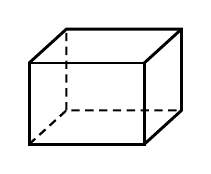
\begin{tikzpicture}[scale=0.86, every node/.style={font=\scriptsize, text=black}]
    \draw[black, line width=1.05pt] (-1.05,-0.75) rectangle (0.65,0.45);
    \draw[black, line width=1.05pt] (0.65,-0.75) -- (1.20,-0.25) -- (1.20,0.95) -- (-0.50,0.95) -- (-1.05,0.45);
    \draw[black, line width=1.05pt] (0.65,0.45) -- (1.20,0.95);
    \draw[black, line width=0.8pt, densely dashed] (-1.05,-0.75) -- (-0.50,-0.25) -- (1.20,-0.25) (-0.50,-0.25) -- (-0.50,0.95);
  \end{tikzpicture}
  &
  % រូបទី២៖ ព្រីសត្រង់ត្រីមុខដេក
  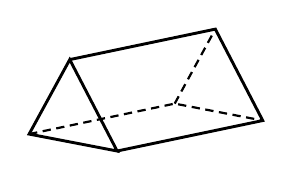
\begin{tikzpicture}[scale=0.86, every node/.style={font=\scriptsize, text=black}]
    \coordinate (A) at (-1.35,-0.55);
    \coordinate (B) at (-0.05,-0.80);
    \coordinate (C) at (-0.75,0.55);
    \coordinate (S) at (2.15,0.45);
    \draw[black, line width=1.05pt] (A) -- (B) -- (C) -- cycle;
    \draw[black, line width=1.05pt] (B) -- ($(B)+(S)$) -- ($(C)+(S)$) -- (C);
    \draw[black, line width=0.8pt, densely dashed] (A) -- ($(A)+(S)$) -- ($(B)+(S)$) ($(A)+(S)$) -- ($(C)+(S)$);
  \end{tikzpicture}
  &
  % រូបទី៣៖ ព្រីសត្រង់បញ្ចមុខ
  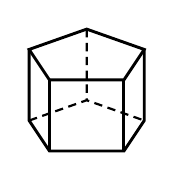
\begin{tikzpicture}[scale=0.86, every node/.style={font=\scriptsize, text=black}]
    \coordinate (P1) at (-0.85,0.65);
    \coordinate (P2) at (0,0.95);
    \coordinate (P3) at (0.85,0.65);
    \coordinate (P4) at (0.55,0.20);
    \coordinate (P5) at (-0.55,0.20);
    \coordinate (D) at (0,-1.05);
    \draw[black, line width=1.05pt] (P1) -- (P2) -- (P3) -- (P4) -- (P5) -- cycle;
    \draw[black, line width=1.05pt] (P1) -- ($(P1)+(D)$) -- ($(P5)+(D)$) -- ($(P4)+(D)$) -- ($(P3)+(D)$) -- (P3);
    \draw[black, line width=1.05pt] (P5) -- ($(P5)+(D)$) (P4) -- ($(P4)+(D)$);
    \draw[black, line width=0.8pt, densely dashed] ($(P1)+(D)$) -- ($(P2)+(D)$) -- ($(P3)+(D)$) (P2) -- ($(P2)+(D)$);
  \end{tikzpicture}
  &
  % រូបទី៤៖ ពីរ៉ាមីតចតុមុខ (Non-Example of Prism!)
  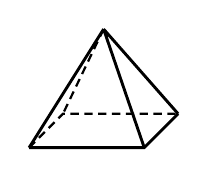
\begin{tikzpicture}[scale=0.86, every node/.style={font=\scriptsize, text=black}]
    \coordinate (E1) at (-1.05,-0.75);
    \coordinate (E2) at (0.65,-0.75);
    \coordinate (E3) at (1.15,-0.25);
    \coordinate (E4) at (-0.55,-0.25);
    \coordinate (V) at (0.05,1.00);
    \draw[black, line width=1.05pt] (E1) -- (E2) -- (E3) (V) -- (E1) (V) -- (E2) (V) -- (E3);
    \draw[black, line width=0.8pt, densely dashed] (E1) -- (E4) -- (E3) (V) -- (E4);
  \end{tikzpicture}
  \\[5pt]
  \footnotesize \textbf{រូបទី១៖} ព្រីស \blank{1.6cm}\par\vspace{3pt}
  \footnotesize មុខខាង៖ \blank{0.7cm} មុខ
  &
  \footnotesize \textbf{រូបទី២៖} បាតជារាង \blank{1.4cm}\par\vspace{3pt}
  \footnotesize មុខខាង៖ \blank{0.7cm} មុខ
  &
  \footnotesize \textbf{រូបទី៣៖} ព្រីស \blank{1.6cm}\par\vspace{3pt}
  \footnotesize មុខខាង៖ \blank{0.7cm} មុខ
  &
  \footnotesize \textbf{រូបទី៤៖} ជាព្រីសឬទេ?\par\vspace{3pt}
  \footnotesize \chkbox\ មែន \hspace{0.15cm} \chkbox\ មិនមែន
\end{tabular}\\[6pt]
$\bullet$ \textbf{សន្និដ្ឋានសម្គាល់បាតព្រីស៖} ទោះបីព្រីសត្រីមុខដាក់ដេកលើដីក៏ដោយ មុខដែលជា «បាតព្រីស» ត្រូវតែជាមុខទាំងពីរដែល \blank{2.6cm} ហើយ \blank{2.4cm} ។

\vspace{16pt}
% --- E2 Explore Part B: 2D Net Unfolding of Worked Example 1 ---
\secbar{ផ្នែកទី១ \enbf{(}ខ\enbf{)} ៖ ការលាតប្លង់ \enbf{2D} នៃព្រីសត្រង់ត្រីមុខ \enbf{---} លំហាត់គំរូទី \enbf{1 (}ទំព័រ ២១៧\enbf{)}}{ការងារជាដៃគូ \en{6 min}}

\noindent
\begin{minipage}[c]{9.2cm}
  \centering
  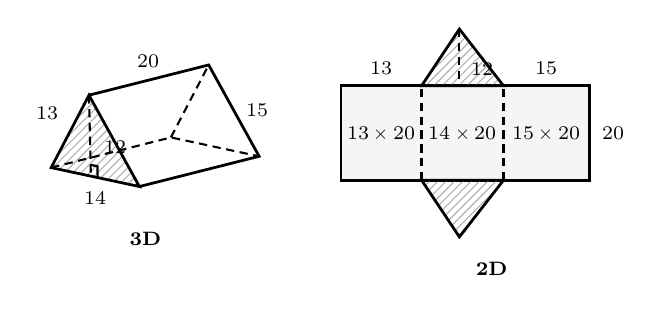
\begin{tikzpicture}[scale=0.80, every node/.style={font=\scriptsize, text=black}]
    % រូប 3D តូចខាងឆ្វេង
    \begin{scope}[shift={(-3.10,0)}]
      \coordinate (A) at (-1.35,-0.55);
      \coordinate (B) at (0.05,-0.85);
      \coordinate (C) at (-0.75,0.60);
      \coordinate (S) at (1.90,0.48);
      \coordinate (H) at ($(A)!0.45!(B)$);
      \fill[pattern=north east lines, pattern color=gray!60] (A) -- (B) -- (C) -- cycle;
      \draw[black, line width=1.0pt] (A) -- (B) -- (C) -- cycle;
      \draw[black, line width=1.0pt] (B) -- ($(B)+(S)$) -- ($(C)+(S)$) -- (C);
      \draw[black, line width=0.75pt, densely dashed] (A) -- ($(A)+(S)$) -- ($(B)+(S)$) ($(A)+(S)$) -- ($(C)+(S)$);
      \draw[black, line width=0.75pt, densely dashed] (C) -- (H);
      \node[right=1.5pt] at ($0.36*(C)+0.64*(H)$) {$12$};
      \rightbox[0.14]{C}{H}{B}
      \node[above left=0.5pt] at ($0.5*(A)+0.5*(C)$) {$13$};
      \node[below=1.5pt] at ($0.5*(A)+0.5*(B)$) {$14$};
      \node[above=1pt] at ($0.5*(C)+0.5*(C)+0.5*(S)$) {$20$};
      \node[right=1pt] at ($0.5*(B)+0.5*(C)+(S)$) {$15$};
      \node at (-0.05,-1.68) {\textbf{រូប \enbf{3D}}};
    \end{scope}

    % រូបគំនូសលាត 2D ខាងស្ដាំ
    \begin{scope}[shift={(2.05,0)}]
      \draw[black, line width=1.05pt, fill=gray!8] (-1.90,-0.75) rectangle (2.05,0.75);
      \draw[black, line width=0.8pt, densely dashed] (-0.62,-0.75) -- (-0.62,0.75);
      \draw[black, line width=0.8pt, densely dashed] (0.68,-0.75) -- (0.68,0.75);
      \fill[pattern=north east lines, pattern color=gray!60] (-0.62,0.75) -- (0.68,0.75) -- (-0.02,1.65) -- cycle;
      \draw[black, line width=1.0pt] (-0.62,0.75) -- (0.68,0.75) -- (-0.02,1.65) -- cycle;
      \draw[black, line width=0.75pt, densely dashed] (-0.02,1.65) -- (-0.02,0.75);
      \node[right=1pt] at (-0.02,1.02) {$12$};
      \fill[pattern=north east lines, pattern color=gray!60] (-0.62,-0.75) -- (0.68,-0.75) -- (-0.02,-1.65) -- cycle;
      \draw[black, line width=1.0pt] (-0.62,-0.75) -- (0.68,-0.75) -- (-0.02,-1.65) -- cycle;
      \node at (-1.26,0) {$13\times 20$};
      \node at (0.03,0) {$14\times 20$};
      \node at (1.36,0) {$15\times 20$};
      \node[right=1pt] at (2.05,0) {$20$};
      \node[above=0.5pt] at (-1.26,0.75) {$13$};
      \node[above=0.5pt] at (1.36,0.75) {$15$};
      \node at (0.08,-2.15) {\textbf{គំនូសលាត \enbf{2D}}};
    \end{scope}
  \end{tikzpicture}
\end{minipage}%
\hfill
\begin{minipage}[c]{9.4cm}
  \textbf{បំពេញការគណនាតាមគំនូសលាត \en{2D} ខាងឆ្វេង៖}\\[6.5pt]
  $1.$ \textbf{ក. ផ្ទៃក្រឡាខាង ($S_l$)៖} ផលបូកផ្ទៃចតុកោណកែងមុខខាងទាំង ៣៖\\[2.5pt]
  \hspace*{0.25cm}$S_l = 13\times 20 + 14\times 20 + 15\times 20 = 260 + \blank{0.9cm} + \blank{0.9cm} = \blank{1.1cm}$\\[3.5pt]
  \hspace*{0.25cm}$\bullet$ បរិមាត្របាត $P = 13 + 14 + 15 = \blank{1.0cm}$\\[3.5pt]
  \hspace*{0.25cm}$\Rightarrow P \times h = \blank{1.0cm} \times 20 = \blank{1.2cm}$ ឯកតាផ្ទៃ!\\[6.5pt]
  $2.$ \textbf{ខ. ផ្ទៃក្រឡាទាំងអស់ ($S_t$)៖} ផ្ទៃបាតត្រីកោណមួយ $B = \dfrac{12\times 14}{2} = \blank{1.0cm}$\\[3.5pt]
  \hspace*{0.25cm}$\Rightarrow S_t = S_l + 2B = \blank{1.1cm} + 2(\blank{1.0cm}) = \blank{1.3cm}$ ឯកតាផ្ទៃ ។
\end{minipage}

\vspace{16pt}
% --- E3 Explain: Definitions & Formula Summary ---
\secbar{ផ្នែកទី២ ៖ និយមន័យធាតុនៃព្រីស និងរូបមន្តផ្ទៃក្រឡាព្រីសត្រង់ \enbf{(E3 - Explain)}}{សង្ខេបរួមគ្នា \en{6 min}}

\begin{tcolorbox}[
  enhanced, sharp corners, colback=white, colframe=black,
  boxrule=0.9pt, boxsep=4pt, top=6.5pt, bottom=6.5pt, left=6pt, right=6pt
]
  $\bullet$ \textbf{ពហុមុខ និងព្រីស (ទំ.២១៦)៖} សូលីតដែលមានមុខច្រើនហៅថា \textbf{\blank{2.3cm}} ។ ព្រីសមានមុខពីរស្របគ្នាហើយប៉ុនគ្នាហៅថា \textbf{\blank{2.3cm}} ($B$) ។ ជ្រុងស្របគ្នាភ្ជាប់កំពូលទាំងពីរនៃបាតហៅថា \textbf{\blank{2.4cm}} ។ ចំពោះ \textbf{ព្រីសត្រង់} ទ្រនុងខាងកែងនឹងបាត ហើយមុខខាងទាំងអស់ជា \textbf{\blank{3.1cm}} ។\\[7pt]
  {\renewcommand{\arraystretch}{1.68}\footnotesize
  \begin{tabular}{|L{4.85cm}|L{5.75cm}|L{6.50cm}|}
    \hline
    \cellcolor{headgray}\textbf{បរិមាណផ្ទៃក្រឡានៃព្រីសត្រង់} & \cellcolor{headgray}\textbf{រូបមន្តគណនា} & \cellcolor{headgray}\textbf{អត្ថន័យនៃអថេរនីមួយៗ} \\
    \hline
    $1.$ ផ្ទៃក្រឡាខាងនៃព្រីស ($S_l$) & $S_l = \blank{1.3cm} \times \blank{1.3cm}$ (ផលបូកមុខខាង) & $P$ ជាបរិមាត្រនៃពហុកោណបាត,\; $h$ ជាកម្ពស់/ទ្រនុងខាង \\
    \hline
    $2.$ ផ្ទៃក្រឡាទាំងអស់នៃព្រីស ($S_t$) & $S_t = S_l + \blank{1.8cm}$ & $B$ ជាផ្ទៃក្រឡានៃបាតមួយ (ត្រូវបូកបាតទាំង \textbf{២}!) \\
    \hline
    $3.$ ប្រលេពីប៉ែតកែង ($l, w, h$) & $S_l = 2(l+w)h$ \;\textbar\; $S_t = S_l + \blank{1.3cm}$ & បាតជាចតុកោណកែង $B = l\times w$ \\
    \hline
    $4.$ ករណីពិសេស៖ គូបជ្រុង $a$ & $S_l = \blank{1.2cm}\,a^2$ \;\textbar\; $S_t = \blank{1.2cm}\,a^2$ & មុខខាងទាំង ៤ និងបាតទាំង ២ សុទ្ធតែជាការេជ្រុង $a$ \\
    \hline
  \end{tabular}}\\[7pt]
  $\bullet$ \textbf{សម្គាល់ (ទំ.២១៦)៖} ព្រីសដែលមានទ្រនុងខាងមិនកែងនឹងបាតហៅថា \textbf{\blank{2.3cm}} (មុខខាងជា \textbf{\blank{2.8cm}}) ។\\[5pt]
  $\bullet$ \textbf{ធនាគារហេតុផល៖}
  \cnum{1} បាតពីរស្របគ្នាប៉ុនគ្នា \;\textbar\;
  \cnum{2} $S_l = P \times h$ \;\textbar\;
  \cnum{3} $S_t = S_l + 2B$ \;\textbar\;
  \cnum{4} $B_{\tri{}}=\frac{1}{2}bh,\; B_{\text{ចតុកោណកែង}}=l\times w$
\end{tcolorbox}

\newpage

% ============================================================================
% ទំព័រទី ២៖ E4 (លំហាត់គំរូទី 2 & ប្រតិបត្តិ ទំ.២១៧) + E5 (Spot-the-Error, លំហាត់ទំ.២២៦ & Exit Check) + កិច្ចការផ្ទះ
% ============================================================================

\secbar{ផ្នែកទី៣ ៖ អនុវត្តគណនាផ្ទៃក្រឡាព្រីសត្រង់ \enbf{---} ទំព័រ ២១៧ \enbf{(E4 - Elaborate)}}{អនុវត្ត \en{10 min}}

\noindent
\begin{minipage}[t]{8.9cm}\vspace{0pt}
  \begin{tcolorbox}[
    enhanced, sharp corners, colback=white, colframe=black, equal height group=rowE4,
    boxrule=0.85pt, boxsep=3pt, top=5pt, bottom=5pt, left=5.5pt, right=5.5pt
  ]
    \textbf{៣.ក លំហាត់គំរូទី \en{2} (ទំ.២១៧)៖ ព្រីសត្រង់ចតុមុខ}\\
    គណនាផ្ទៃក្រឡាខាង $S_l$ និងផ្ទៃក្រឡាទាំងអស់ $S_t$ នៃព្រីសត្រង់ចតុមុខខាងក្រោម៖
    \begin{center}
      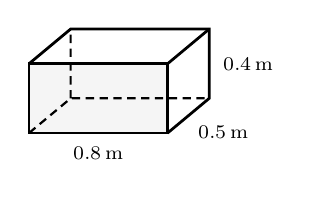
\begin{tikzpicture}[scale=0.88, every node/.style={font=\scriptsize, text=black}]
        \draw[black, line width=1.0pt, fill=gray!8] (-1.20,-0.65) rectangle (0.80,0.35);
        \draw[black, line width=1.0pt] (0.80,-0.65) -- (1.40,-0.15) -- (1.40,0.85) -- (-0.60,0.85) -- (-1.20,0.35);
        \draw[black, line width=1.0pt] (0.80,0.35) -- (1.40,0.85);
        \draw[black, line width=0.8pt, densely dashed] (-1.20,-0.65) -- (-0.60,-0.15) -- (1.40,-0.15) (-0.60,-0.15) -- (-0.60,0.85);
        \node[below=1.5pt] at (-0.20,-0.65) {$0.8\unit{m}$};
        \node[below right=0pt] at (1.10,-0.40) {$0.5\unit{m}$};
        \node[right=1.5pt] at (1.40,0.35) {$0.4\unit{m}$};
      \end{tikzpicture}
    \end{center}
    $\bullet$ \textbf{ក. ផ្ទៃក្រឡាខាង ($S_l$)៖}\\[2pt]
    \hspace*{0.2cm}$S_l = (0.8\times 0.4)\times 2 + (0.5\times 0.4)\times 2$\\[4pt]
    \hspace*{0.62cm}$= \blank{1.3cm} + \blank{1.3cm} = \blank{1.5cm}\unit{m}^2$ ។\\[5pt]
    $\bullet$ \textbf{ខ. ផ្ទៃក្រឡាទាំងអស់ ($S_t$)៖}\\[2pt]
    \hspace*{0.2cm}$2B = (0.8\times 0.5)\times 2 = \blank{1.4cm}\unit{m}^2$\\[4pt]
    \hspace*{0.2cm}$\Rightarrow S_t = S_l + 2B = \blank{1.3cm} + \blank{1.3cm} = \blank{1.5cm}\unit{m}^2$ ។
  \end{tcolorbox}
\end{minipage}%
\hfill
\begin{minipage}[t]{9.9cm}\vspace{0pt}
  \begin{tcolorbox}[
    enhanced, sharp corners, colback=white, colframe=black, equal height group=rowE4,
    boxrule=0.85pt, boxsep=3pt, top=5pt, bottom=5pt, left=5.5pt, right=5.5pt
  ]
    \textbf{៣.ខ ប្រតិបត្តិ (ទំ.២១៧)៖ គណនា $S_l$ និង $S_t$ នៃរូប ក និង រូប ខ}
    \begin{center}
      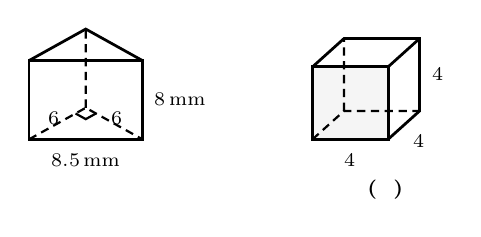
\begin{tikzpicture}[scale=0.80, every node/.style={font=\scriptsize, text=black}]
        \begin{scope}[shift={(-2.15,0)}]
          \coordinate (L1) at (-0.95,-0.65);
          \coordinate (R1) at (0.85,-0.65);
          \coordinate (M1) at (-0.05,-0.15);
          \coordinate (L2) at (-0.95,0.60);
          \coordinate (R2) at (0.85,0.60);
          \coordinate (M2) at (-0.05,1.10);
          \draw[black, line width=1.0pt] (L1) -- (R1) -- (R2) -- (L2) -- cycle;
          \draw[black, line width=1.0pt] (L2) -- (M2) -- (R2);
          \draw[black, line width=0.8pt, densely dashed] (L1) -- (M1) -- (R1) (M1) -- (M2);
          \rightbox[0.18]{L1}{M1}{R1}
          \node[below=1.5pt] at (-0.05,-0.65) {$8.5\unit{mm}$};
          \node[right=1pt] at (0.85,-0.02) {$8\unit{mm}$};
          \node at (-0.55,-0.32) {$6$};
          \node at (0.45,-0.32) {$6$};
          \node at (-0.05,-1.45) {\textbf{រូប ក}};
        \end{scope}
        \begin{scope}[shift={(2.15,0)}]
          \draw[black, line width=1.0pt, fill=gray!8] (-0.75,-0.65) rectangle (0.45,0.50);
          \draw[black, line width=1.0pt] (0.45,-0.65) -- (0.95,-0.20) -- (0.95,0.95) -- (-0.25,0.95) -- (-0.75,0.50);
          \draw[black, line width=1.0pt] (0.45,0.50) -- (0.95,0.95);
          \draw[black, line width=0.8pt, densely dashed] (-0.75,-0.65) -- (-0.25,-0.20) -- (0.95,-0.20) (-0.25,-0.20) -- (-0.25,0.95);
          \node[below=1.5pt] at (-0.15,-0.65) {$4$};
          \node[below right=0pt] at (0.70,-0.42) {$4$};
          \node[right=1pt] at (0.95,0.38) {$4$};
          \node at (0.10,-1.45) {\textbf{រូប ខ (គូប)}};
        \end{scope}
      \end{tikzpicture}
    \end{center}
    \vspace{-2pt}
    $\bullet$ \textbf{រូប ក៖} $P = 6 + 6 + 8.5 = \blank{1.2cm}\unit{mm}$\\[3.5pt]
    \hspace*{0.25cm}$S_l = \blank{1.2cm}\times 8 = \blank{1.4cm}\unit{mm}^2$\\[3.5pt]
    \hspace*{0.25cm}$2B = 2\times\dfrac{6\times 6}{2} = \blank{1.1cm}\unit{mm}^2 \Rightarrow S_t = \blank{1.4cm}\unit{mm}^2$ ។\\[4.5pt]
    $\bullet$ \textbf{រូប ខ៖} $S_l = 4\times 4^2 = \blank{1.2cm}$;\; $S_t = 6\times 4^2 = \blank{1.2cm}$ ឯកតាផ្ទៃ ។
  \end{tcolorbox}
\end{minipage}

\vspace{7pt}
% --- E5 Evaluate: Spot-the-Error + Exercise 2a + Exit Check ---
\secbar{ផ្នែកទី៤ ៖ វាយតម្លៃ \enbf{---} វិនិច្ឆ័យកំហុស, លំហាត់ទំព័រ ២២៦ និង \enbf{Exit Check (E5)}}{ធ្វើដោយឯករាជ្យ \en{10 min}}

\noindent
\begin{minipage}[t]{10.3cm}\vspace{0pt}
  \begin{tcolorbox}[
    enhanced, sharp corners, colback=white, colframe=black, equal height group=rowE5,
    boxrule=0.85pt, boxsep=3pt, top=5pt, bottom=5pt, left=5.5pt, right=5.5pt
  ]
    \textbf{៤.ក ការវិនិច្ឆ័យកំហុស និងលំហាត់អនុវត្ត (ទំ.២២៦)៖}\\[4.5pt]
    $1.$ \textbf{ចាប់កំហុស (លំហាត់ទី១ក៖ ប្រលេពីប៉ែតកែង $l=13, w=6, h=10\unit{cm}$)៖}\\
    សិស្សម្នាក់គណនា៖ $S_l = 2(13+6)\times 10 = 380\unit{cm}^2$ រួចដាក់៖\\[2pt]
    \hspace*{0.3cm}$S_t = 380 + (13\times 6) = 380 + 78 = 458\unit{cm}^2$ ។\\[4pt]
    $\bullet$ តើសិស្សនេះខុសត្រង់ណា? \blank{5.5cm}\\[5pt]
    $\bullet$ ចម្លើយត្រឹមត្រូវ៖ $S_t = 380 + 2(\blank{1.0cm}) = \blank{1.6cm}\unit{cm}^2$ ។\\[7pt]
    $2.$ \textbf{លំហាត់ទី២ក (ទំ.២២៦)៖} គណនាផ្ទៃក្រឡាខាងនៃព្រីសត្រង់ត្រីមុខដែលមានជ្រុងបាត $a=3\unit{cm},\; b=5\unit{cm},\; c=7\unit{cm}$ និងកម្ពស់ព្រីស $h=10\unit{cm}$៖\\[4.5pt]
    \hspace*{0.2cm}$P = \blank{0.8cm} + \blank{0.8cm} + \blank{0.8cm} = \blank{1.2cm}\unit{cm}$\\[4.5pt]
    \hspace*{0.2cm}$\Rightarrow S_l = P \times h = \blank{1.1cm} \times \blank{1.1cm} = \blank{1.6cm}\unit{cm}^2$ ។
  \end{tcolorbox}
\end{minipage}%
\hfill
\begin{minipage}[t]{8.5cm}\vspace{0pt}
  \begin{tcolorbox}[
    enhanced, sharp corners, colback=white, colframe=black, equal height group=rowE5,
    boxrule=0.85pt, boxsep=3pt, top=5pt, bottom=5pt, left=5.5pt, right=5.5pt
  ]
    \textbf{៤.ខ សំណួរត្រួតពិនិត្យរហ័ស (\en{Exit Check})៖}\\
    គូសវង់ជុំវិញអក្សរនៃចម្លើយត្រឹមត្រូវតែមួយគត់៖\\[6pt]
    \textbf{សំណួរទី១ (បេសកកម្ម \en{E1})៖} ចំពោះព្រីសត្រង់ត្រីមុខដេក តើមុខណាជា «បាតព្រីស»?\\[2pt]
    \hspace*{0.15cm}\textbf{ក.} មុខចតុកោណកែងក្រោម \hspace{0.2cm} \textbf{ខ.} មុខត្រីកោណពីរស្របគ្នា\\
    \hspace*{0.15cm}\textbf{គ.} មុខធំជាងគេបំផុត\\[7pt]
    \textbf{សំណួរទី២៖} រូបមន្តផ្ទៃក្រឡាទាំងអស់នៃព្រីសត្រង់គឺ៖\\[2pt]
    \hspace*{0.15cm}\textbf{ក.} $S_t = S_l + B$ \hspace{0.35cm} \textbf{ខ.} $S_t = 2S_l + B$ \hspace{0.35cm} \textbf{គ.} $S_t = S_l + 2B$\\[7pt]
    \textbf{សំណួរទី៣៖} ព្រីសត្រង់ចតុមុខមានបរិមាត្របាត $P=16\unit{cm}$ និងកម្ពស់ $h=5\unit{cm}$ មានផ្ទៃក្រឡាខាង $S_l$ ស្មើនឹង៖\\[2pt]
    \hspace*{0.15cm}\textbf{ក.} $80\unit{cm}^2$ \hspace{0.55cm} \textbf{ខ.} $21\unit{cm}^2$ \hspace{0.55cm} \textbf{គ.} $40\unit{cm}^2$
  \end{tcolorbox}
\end{minipage}

\vspace{7pt}
% --- Step 5 Homework Box ---
\secbar{ផ្នែកទី៥ ៖ កិច្ចការផ្ទះ និងបណ្ដាំផ្ញើ \enbf{(}ទំព័រ ២២៦\enbf{--}២២៧ លំហាត់ទី១ខ និងទី៣\enbf{)}}{ធ្វើនៅផ្ទះក្នុងសៀវភៅសរសេរ}

\begin{tcolorbox}[
  enhanced, sharp corners, colback=panelgray, colframe=black,
  boxrule=0.85pt, boxsep=3.5pt, top=5.5pt, bottom=5.5pt, left=6pt, right=6pt
]
  \begin{minipage}[c]{13.8cm}
    $1.$ \textbf{លំហាត់ទី១ខ (ទំ.២២៦)៖} គណនាផ្ទៃក្រឡាសរុបនៃប្រលេពីប៉ែតកែងដែលមាន $l=12\unit{mm},\; w=8\unit{mm},\; h=13\unit{mm}$ ។\\[3.5pt]
    $2.$ \textbf{លំហាត់ទី៣ (ទំ.២២៧)៖} គេមានព្រីសត្រង់ត្រីមុខដែលមានបាតជាត្រីកោណសមបាត ($17, 17, 16$) និងទ្រនុងខាង $11$ (ដូចរូបស្ដាំ) ។ ចូរគណនា៖ \textbf{ក.} ផ្ទៃក្រឡាខាង $S_l$ \; \textbf{ខ.} ផ្ទៃក្រឡាបាតមួយ $B$ \textit{(គន្លឹះពីតាករ៖ $h_{\text{បាត}}=\sqrt{17^2-8^2}=15$)} \; \textbf{គ.} ផ្ទៃក្រឡាសរុប $S_t$ ។\\[3.5pt]
    $3.$ \textbf{អានមេរៀនបន្ទាប់៖} ១៧.១ ផ្ទៃក្រឡាខាងនិងផ្ទៃក្រឡាទាំងអស់នៃពីរ៉ាមីត (ទំ.២១៨\,\en{--}\,២២០) ។
  \end{minipage}%
  \hfill
  \begin{minipage}[c]{4.2cm}
    \centering
    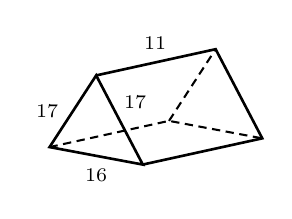
\begin{tikzpicture}[scale=0.74, every node/.style={font=\scriptsize, text=black}]
      \coordinate (A) at (-1.45,-0.55);
      \coordinate (B) at (0.15,-0.85);
      \coordinate (C) at (-0.65,0.68);
      \coordinate (S) at (2.05,0.45);
      \draw[black, line width=0.95pt] (A) -- (B) -- (C) -- cycle;
      \draw[black, line width=0.95pt] (B) -- ($(B)+(S)$) -- ($(C)+(S)$) -- (C);
      \draw[black, line width=0.75pt, densely dashed] (A) -- ($(A)+(S)$) -- ($(B)+(S)$) ($(A)+(S)$) -- ($(C)+(S)$);
      \node[left=1.5pt] at ($0.5*(A)+0.5*(C)$) {$17$};
      \node[above right=-1pt] at ($0.45*(B)+0.55*(C)$) {$17$};
      \node[below=1pt] at ($0.5*(A)+0.5*(B)$) {$16$};
      \node[above=1pt] at ($0.5*(C)+0.5*(C)+0.5*(S)$) {$11$};
    \end{tikzpicture}
  \end{minipage}
\end{tcolorbox}

\end{document}
